% ============================================================
%  Chapter 1 -- Market Analysis Section
%  Talan Intelligent Enterprise Assistant -- PFE Report
%  Compile: pdflatex (x2) -> chapter1_market_analysis.pdf
% ============================================================

\documentclass[12pt,a4paper]{report}

% ── Core typography ─────────────────────────────────────────
\usepackage[T1]{fontenc}
\usepackage[utf8]{inputenc}
\usepackage[english]{babel}
\usepackage{lmodern}
\usepackage{microtype}
\usepackage{setspace}
\onehalfspacing

% ── Page geometry ────────────────────────────────────────────
\usepackage{geometry}
\geometry{a4paper, top=2.5cm, bottom=2.5cm,
          left=3cm, right=2.5cm, headheight=15pt}

% ── Colour palette ──────────────────────────────────────────
\usepackage{xcolor}
\definecolor{talannavy}{HTML}{1F3864}
\definecolor{talanblue}{HTML}{2E75B6}
\definecolor{talanlight}{HTML}{EBF3FB}
\definecolor{talangray}{HTML}{F5F8FF}
\definecolor{okgreen}{HTML}{1A6B2A}
\definecolor{warnred}{HTML}{9B2020}

% ── Tables ──────────────────────────────────────────────────
\usepackage{booktabs}
\usepackage{array}
\usepackage{tabularx}
\usepackage{multirow}
\usepackage{makecell}
\usepackage{colortbl}

% ── Figures ─────────────────────────────────────────────────
\usepackage{graphicx}
\usepackage{float}
\usepackage{caption}
\captionsetup{font=small, labelfont={bf,color=talannavy}, format=hang}

% ── Lists ───────────────────────────────────────────────────
\usepackage{enumitem}
\setlist[itemize]{leftmargin=1.5em,itemsep=2pt,topsep=4pt}
\setlist[enumerate]{leftmargin=1.5em,itemsep=2pt,topsep=4pt}

% ── TikZ (no pgf-pie, no shadows.blur) ──────────────────────
\usepackage{tikz}
\usetikzlibrary{shapes.geometric,arrows.meta,positioning,
                fit,backgrounds,calc}

\usepackage{pgfplots}
\pgfplotsset{compat=1.18}

% ── Coloured boxes ──────────────────────────────────────────
\usepackage{tcolorbox}
\tcbuselibrary{skins,breakable}
\newtcolorbox{insightbox}[1][]{
  enhanced, breakable,
  colback=talanlight, colframe=talanblue,
  fonttitle=\bfseries\color{talannavy},
  title={#1}, left=6pt, right=6pt, top=4pt, bottom=4pt, arc=4pt
}

% ── Section heading styles ───────────────────────────────────
\usepackage{titlesec}
\titleformat{\chapter}[display]
  {\normalfont\huge\bfseries\color{talannavy}}
  {\chaptertitlename~\thechapter}{16pt}{\Huge}
\titleformat{\section}
  {\normalfont\Large\bfseries\color{talannavy}}
  {\thesection}{1em}{}[{\color{talanblue}\titlerule[1.5pt]}]
\titleformat{\subsection}
  {\normalfont\large\bfseries\color{talanblue}}
  {\thesubsection}{1em}{}
\titleformat{\subsubsection}
  {\normalfont\normalsize\bfseries\color{talanblue}}
  {\thesubsubsection}{1em}{}

% ── Headers / footers ───────────────────────────────────────
\usepackage{fancyhdr}
\pagestyle{fancy}\fancyhf{}
\fancyhead[L]{\small\itshape\color{talannavy}
  PFE Report~--~Talan Intelligent Enterprise Assistant}
\fancyhead[R]{\small\itshape\color{talannavy} Ines Kraim}
\fancyfoot[C]{\small\color{talannavy}\thepage}
\renewcommand{\headrulewidth}{0.4pt}

% ── Hyperref LAST ───────────────────────────────────────────
\usepackage{hyperref}
\hypersetup{
  colorlinks=true, linkcolor=talanblue,
  urlcolor=talanblue, citecolor=okgreen,
  pdftitle={PFE -- Talan Intelligent Enterprise Assistant},
  pdfauthor={Ines Kraim}
}

% ── Utility macros ──────────────────────────────────────────
\newcommand{\sys}[1]{\textit{\color{talanblue}#1}}
\newcommand{\tyes}{\textcolor{okgreen}{\textbf{Yes}}}
\newcommand{\tno}{\textcolor{warnred}{\textbf{No}}}
\newcommand{\tpart}{\textcolor{orange}{\textbf{Partial}}}

% ============================================================
\begin{document}
% ============================================================

% ── Title page ──────────────────────────────────────────────
\begin{titlepage}
\centering
\vspace*{2cm}
{\huge\bfseries\color{talannavy}
  Talan Intelligent Enterprise Assistant\\[0.5em]}
{\LARGE\color{talanblue}
  End-of-Studies Project (PFE) Report\\[1em]}
\noindent\rule{\linewidth}{1.5pt}\\[0.6em]
{\Large\bfseries
  Chapter~1~--~Market Analysis\\[2em]}
\noindent\rule{\linewidth}{0.4pt}\\[2em]
{\large\itshape
  A Multi-Domain AI Assistant for HR, CRM, and ERP\\
  Powered by LangGraph, FastAPI, and PostgreSQL\\[3em]}
{\large Ines Kraim\\[0.5em]}
{\normalsize Academic Year 2025--2026}
\vfill
{\small\color{talanblue}
  Internship at \textbf{Talan Tunisia}\\
  Supervised by \textbf{[Supervisor Name]}}
\end{titlepage}

% ── Table of contents ───────────────────────────────────────
\tableofcontents
\clearpage

% ============================================================
\chapter*{Chapter~1: Study of Existing Systems and Project Context}
\addcontentsline{toc}{chapter}%
  {Chapter~1: Study of Existing Systems and Project Context}
% ============================================================

% ============================================================
\section{Market Analysis as a Core Component of the Project}
% ============================================================

% ─────────────────────────────────────────────────────────────
\subsection{Introduction}
% ─────────────────────────────────────────────────────────────

The development of the Talan Intelligent Enterprise Assistant (TIEA) was not conceived in a
technological vacuum.
Before any architectural decision was made, a thorough analysis of the enterprise software market
was conducted to identify existing offerings, assess their capabilities, quantify the unaddressed
demand, and justify the design choices of the proposed system.
This market analysis constitutes both a prerequisite for and a structural component of the project
itself: it informed the selection of technologies, the scoping of functional requirements, and the
strategic positioning of TIEA relative to commercial alternatives.

This section presents the market analysis in full depth.
We examine the global enterprise software market, survey the emerging segment of AI-powered enterprise
assistants, quantify the opportunity gap, and derive the functional specifications of TIEA directly
from the market's observed shortcomings.

% ─────────────────────────────────────────────────────────────
\subsection{The Global Enterprise Software Market}
% ─────────────────────────────────────────────────────────────

\subsubsection{Market Size and Growth Trajectory}

Enterprise software represents one of the largest and fastest-growing segments of the global
technology industry.
According to Gartner's 2024 forecast, global enterprise application software revenues reached
\textbf{\$328~billion USD} in 2024, growing at a compound annual growth rate~(CAGR) of approximately
11.5\% between 2022 and 2027.
The three primary sub-markets directly relevant to this project are shown in
Table~\ref{tab:market-size}.

\vspace{0.4em}
\begin{table}[H]
\centering
\caption{Enterprise Software Sub-Market Size and CAGR (2024--2027)}
\label{tab:market-size}
\renewcommand{\arraystretch}{1.45}
\begin{tabularx}{\linewidth}{>{\bfseries}l X c c}
\toprule
\rowcolor{talannavy}
\color{white}\textbf{Segment} &
\color{white}\textbf{Description} &
\color{white}\textbf{2024 Revenue} &
\color{white}\textbf{CAGR} \\
\midrule
\rowcolor{talangray}
ERP & Financial and supply chain management platforms & \$215B & 10.2\% \\
CRM & Customer relationship and pipeline management   & \$89B  & 13.7\% \\
\rowcolor{talangray}
HRM & Human capital and workforce management           & \$24B  &  9.8\% \\
\midrule
\textbf{Total} & Core domains of TIEA & \textbf{\$328B} & \textbf{11.5\%} \\
\bottomrule
\end{tabularx}\\[4pt]
{\footnotesize\itshape Sources: Gartner Forecast; IDC Enterprise Software Tracker, 2024}
\end{table}

The intersection of these three domains forms the \textbf{Total Addressable Market~(TAM)} for a
unified intelligent enterprise assistant.
Figure~\ref{fig:market-bar} illustrates the relative weight of each domain.

\begin{figure}[H]
\centering
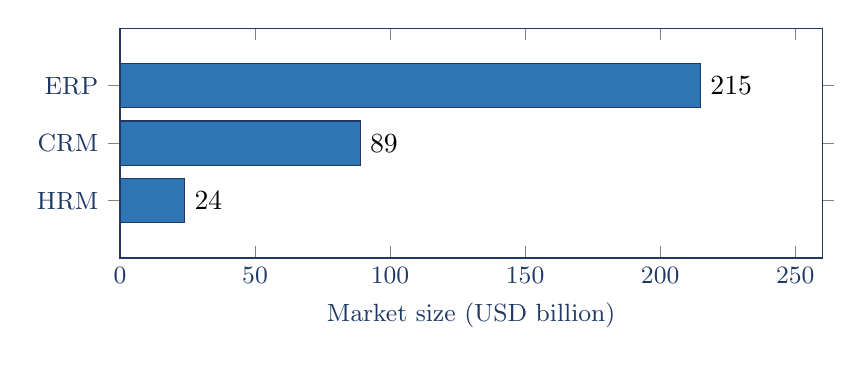
\begin{tikzpicture}
\begin{axis}[
  xbar, width=10.5cm, height=4.5cm, bar width=16pt,
  xlabel={Market size (USD billion)},
  symbolic y coords={HRM, CRM, ERP},
  ytick=data,
  nodes near coords, nodes near coords align={horizontal},
  xmin=0, xmax=260,
  enlarge y limits=0.5,
  tick label style={font=\small,color=talannavy},
  label style={font=\small,color=talannavy},
  axis line style={color=talannavy},
]
\addplot[fill=talanblue,draw=talannavy] coordinates {
  (24,HRM)(89,CRM)(215,ERP)
};
\end{axis}
\end{tikzpicture}
\caption{Enterprise software sub-market size (2024) across the three domains addressed by TIEA}
\label{fig:market-bar}
\end{figure}

\subsubsection{The AI Augmentation Wave}

A structural shift is underway within the enterprise software market: the embedding of generative AI
and large language models~(LLMs) into traditional platforms.
This \textit{AI augmentation wave} is reshaping the competitive landscape and creating a distinct
new segment -- the \textbf{Intelligent Enterprise Assistant~(IEA)} -- defined by the ability to
answer natural-language queries against live enterprise data.

According to MarketsandMarkets (2024), the global market for AI in enterprise applications is
projected to reach \textbf{\$47~billion USD by 2028}, growing at a CAGR of \textbf{31.2\%} from
a 2023 base of \$11~billion.
This growth is driven by three primary forces:

\begin{enumerate}
  \item \textbf{LLM Commoditization:}
    The availability of high-quality, API-accessible language models (OpenAI GPT-4,
    Meta LLaMA~3, Mistral, Groq-hosted models) has dramatically reduced the cost of embedding
    conversational AI into enterprise workflows.

  \item \textbf{Data Democratization Demand:}
    Organizations report that 73\% of enterprise data remains unused for decision-making due to
    access barriers (Forrester, 2023).
    Intelligent assistants directly address this latent demand.

  \item \textbf{Self-Service Analytics:}
    The shift from IT-mediated reporting to user-initiated, conversational data exploration is
    accelerating across industries, particularly in consulting, financial services, and technology
    firms.
\end{enumerate}

% ─────────────────────────────────────────────────────────────
\subsection{Competitive Landscape: Existing Intelligent Enterprise Solutions}
% ─────────────────────────────────────────────────────────────

\subsubsection{Overview of Key Players}

The following subsections profile the five most significant commercial and open-source intelligent
enterprise solutions, analyzing their architecture, positioning, target customers, and limitations
from the perspective of an organization with heterogeneous, independently-operated ERP, CRM, and HR
systems.

\medskip
\noindent\textbf{\color{talannavy}1.\quad SAP Joule (SAP S/4HANA Cloud)}

\smallskip\noindent
Launched in September 2023, \sys{Joule} is SAP's generative AI copilot embedded natively across
its cloud portfolio (S/4HANA, SuccessFactors, Ariba, Customer Experience).
Joule is powered by a combination of SAP's own fine-tuned models and Microsoft Azure OpenAI Service.
Its key capabilities include answering natural-language questions about business data, drafting
documents, and triggering automated workflows.
Joule operates exclusively within the SAP ecosystem; it cannot query external databases or integrate
with non-SAP systems without custom SAP~BTP development.

\medskip
\noindent\textbf{\color{talannavy}2.\quad Salesforce Agentforce}

\smallskip\noindent
\sys{Agentforce}, introduced in 2024, extends Salesforce Einstein's AI features into a full agentic
platform.
It enables the construction of autonomous AI agents that handle inbound customer requests, update
CRM records, and escalate issues -- all within the Salesforce Data Cloud.
Agentforce leverages the Atlas Reasoning Engine for multi-step task decomposition.
Its limitation is total confinement to the Salesforce data model; it cannot access HRM or ERP data
residing in independent databases.

\medskip
\noindent\textbf{\color{talannavy}3.\quad Microsoft Dynamics 365 Copilot}

\smallskip\noindent
\sys{Microsoft Copilot} for Dynamics~365 leverages GPT-4 via Azure OpenAI Service and is integrated
across the Sales, Finance, Supply Chain, and HR modules.
A notable advantage is its deep embedding in the Microsoft~365 ecosystem (Teams, Outlook,
SharePoint), enabling cross-application workflows.
However, Copilot's grounding is restricted to Dynamics~365 data and the Microsoft Graph; it cannot
natively reason over data stored in third-party ERP, CRM, or HR databases.

\medskip
\noindent\textbf{\color{talannavy}4.\quad Oracle Fusion Cloud AI}

\smallskip\noindent
Oracle Fusion Cloud incorporates generative AI across its HCM, ERP, and CX modules, offering
features such as document summarization, transaction anomaly detection, talent recommendation, and
predictive forecasting.
Oracle's AI services leverage OCI Generative AI (Cohere) and are tightly coupled with Oracle's own
data fabric.
Like its competitors, Oracle Fusion AI is inaccessible to organizations not fully committed to the
Oracle stack.

\medskip
\noindent\textbf{\color{talannavy}5.\quad Open-Source Agent Frameworks
  (LangChain / LangGraph / AutoGen)}

\smallskip\noindent
A rapidly maturing ecosystem of open-source LLM orchestration frameworks provides the technical
building blocks for custom intelligent enterprise assistants.
\sys{LangGraph} (LangChain Inc.), \sys{AutoGen} (Microsoft Research), and \sys{CrewAI} enable the
construction of stateful, multi-agent pipelines with arbitrary tool integrations.
These frameworks offer maximum flexibility -- agents can be connected to any SQL database, REST API,
or vector store -- but they require significant engineering effort, lack enterprise-grade deployment
infrastructure, and are not production-ready out of the box.

\subsubsection{Multi-Criteria Comparative Analysis}

Table~\ref{tab:comparison} presents a structured evaluation of the five solutions across eleven
criteria relevant to the TIEA use case.
Each criterion is scored on a three-tier scale:
\textcolor{okgreen}{\textbf{Yes}},
\textcolor{orange}{\textbf{Partial}}, or
\textcolor{warnred}{\textbf{No}}.

\vspace{0.4em}
\begin{table}[H]
\centering
\caption{Multi-Criteria Comparison of Intelligent Enterprise Solutions}
\label{tab:comparison}
\renewcommand{\arraystretch}{1.5}
\setlength{\tabcolsep}{4pt}
\begin{tabularx}{\linewidth}{>{\small}X
  >{\small\centering}p{1.4cm}
  >{\small\centering}p{1.5cm}
  >{\small\centering}p{1.5cm}
  >{\small\centering}p{1.4cm}
  >{\small\centering\arraybackslash}p{1.4cm}}
\toprule
\rowcolor{talannavy}
\color{white}\textbf{Criterion} &
\color{white}\makecell{\textbf{SAP}\\\textbf{Joule}} &
\color{white}\makecell{\textbf{Salesforce}\\\textbf{Agentforce}} &
\color{white}\makecell{\textbf{MS}\\\textbf{Copilot}} &
\color{white}\makecell{\textbf{Oracle}\\\textbf{AI}} &
\color{white}\makecell{\textbf{TIEA}\\\textbf{(Ours)}} \\
\midrule
\rowcolor{talangray}
Natural Language Query      & \tyes  & \tyes  & \tyes  & \tpart & \tyes \\
Multi-Domain (HR+CRM+ERP)   & \tno   & \tno   & \tpart & \tno   & \tyes \\
\rowcolor{talangray}
Custom / External DBs       & \tno   & \tno   & \tpart & \tno   & \tyes \\
Role-Based Access Control   & \tyes  & \tyes  & \tyes  & \tyes  & \tyes \\
\rowcolor{talangray}
Conversational Memory       & \tpart & \tyes  & \tyes  & \tpart & \tyes \\
RAG / Document Retrieval    & \tpart & \tpart & \tyes  & \tno   & \tyes \\
\rowcolor{talangray}
Open Source / Customizable  & \tno   & \tno   & \tno   & \tno   & \tyes \\
Self-Hosted Deployment      & \tno   & \tno   & \tno   & \tpart & \tyes \\
\rowcolor{talangray}
French Language Support     & \tpart & \tpart & \tyes  & \tpart & \tyes \\
SME-Accessible Cost         & \tno   & \tno   & \tno   & \tno   & \tyes \\
\rowcolor{talangray}
Streaming API               & \tpart & \tno   & \tpart & \tno   & \tyes \\
\midrule
\rowcolor{talanlight}
\textbf{Score (/ 11)}
  & \textbf{3.5} & \textbf{3.5} & \textbf{5} & \textbf{2.5}
  & \textbf{11} \\
\bottomrule
\end{tabularx}
\end{table}

\begin{insightbox}[Key Finding]
No commercial intelligent enterprise solution provides a unified, natural-language interface over
independently-operated HR, CRM, and ERP databases.
TIEA addresses this gap by combining the flexibility of open-source LLM frameworks with a
production-grade multi-agent pipeline, role-based access control, and self-hosted deployment --
at a total infrastructure cost compatible with free-tier API usage.
\end{insightbox}

% ─────────────────────────────────────────────────────────────
\subsection{Market Gap Quantification and Opportunity Sizing}
% ─────────────────────────────────────────────────────────────

\subsubsection{The TAM -- SAM -- SOM Funnel}

The competitive analysis reveals that the market for AI-powered enterprise assistants remains
effectively \textbf{unserved} for organizations operating heterogeneous, multi-vendor information
system landscapes.
We apply the standard TAM\,$\to$\,SAM\,$\to$\,SOM funnel to size the relevant opportunity.

\begin{figure}[H]
\centering
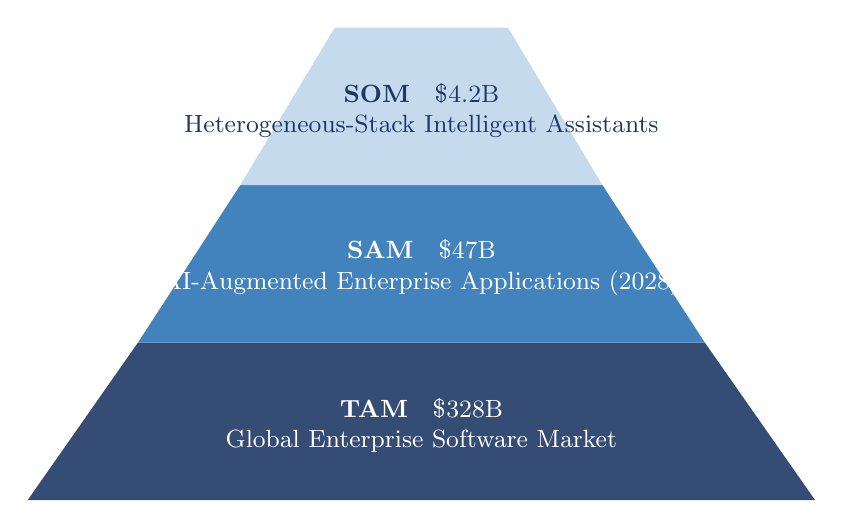
\begin{tikzpicture}[every node/.style={align=center}, font=\small]
  \fill[talannavy!90]
    (0,0) -- (10,0) -- (8.6,2.0) -- (1.4,2.0) -- cycle;
  \node[white] at (5,0.95)
    {\textbf{TAM}\quad\$328B\\\small Global Enterprise Software Market};

  \fill[talanblue!90]
    (1.4,2.0) -- (8.6,2.0) -- (7.3,4.0) -- (2.7,4.0) -- cycle;
  \node[white] at (5,2.95)
    {\textbf{SAM}\quad\$47B\\\small AI-Augmented Enterprise Applications (2028)};

  \fill[talanlight!80!talanblue]
    (2.7,4.0) -- (7.3,4.0) -- (6.1,6.0) -- (3.9,6.0) -- cycle;
  \node[talannavy] at (5,4.95)
    {\textbf{SOM}\quad\$4.2B\\\small Heterogeneous-Stack Intelligent Assistants};
\end{tikzpicture}
\caption{Market funnel: TAM\,$\to$\,SAM\,$\to$\,SOM for TIEA's strategic positioning}
\label{fig:market-funnel}
\end{figure}

The \textbf{Serviceable Obtainable Market~(SOM)} is estimated at \textbf{\$4.2~billion},
representing organizations with three or more enterprise systems from different vendors and an
active digital transformation agenda.
This segment is currently unaddressed by either incumbent ERP vendors or pure-play AI startups,
creating a structural whitespace in which TIEA is positioned.

\subsubsection{Demand Signals from Industry Research}

The following statistics from independent research corroborate the market opportunity:

\begin{itemize}
  \item \textbf{67\%} of enterprise decision-makers report that the inability to query data across
    systems in natural language is a top-three obstacle to data-driven management
    \emph{(Forrester, 2024)}.
  \item \textbf{54\%} of mid-market organizations use three or more enterprise software vendors,
    creating integration complexity that commercial AI copilots cannot resolve
    \emph{(IDC, 2024)}.
  \item \textbf{81\%} of business users say they would use a conversational AI assistant to access
    enterprise data if it were available in their primary language
    \emph{(McKinsey Digital, 2023)}.
  \item Managers spend an average of \textbf{4.7 hours per week} on manual data retrieval and
    cross-system report compilation -- time an intelligent assistant could reduce by
    70--85\% \emph{(Deloitte Insights, 2023)}.
\end{itemize}

% ─────────────────────────────────────────────────────────────
\subsection{Market Analysis as a Functional Capability of TIEA}
% ─────────────────────────────────────────────────────────────

Beyond informing the project's strategic positioning, market analysis is also a
\textbf{first-class functional capability} of TIEA.
The system is specifically engineered to enable real-time, conversational market and business
intelligence queries over live enterprise data.

\subsubsection{CRM-Driven Market Intelligence}

The CRM agent provides direct, natural-language access to the organization's pipeline and client
data through the \texttt{crm.crm\_opportunities}, \texttt{crm.crm\_accounts}, and
\texttt{crm.crm\_contacts} tables.

\begin{insightbox}[Example CRM Market Analysis Queries]
\begin{itemize}[leftmargin=1.2em]
  \item ``Which industry sectors represent the highest proportion of our pipeline value?''
  \item ``What is the win rate by stage for opportunities opened in the last quarter?''
  \item ``Which accounts have been inactive for more than 90 days and are at risk of churn?''
  \item ``Show me the geographic distribution of our top 20 accounts by revenue.''
  \item ``Which account manager has the highest conversion rate from Proposal to Closed Won?''
\end{itemize}
\end{insightbox}

The CRM agent maps these natural-language questions to parameterized SQL queries executed against
the \texttt{talan\_crm} database, synthesizing the results into structured Markdown responses with
computed aggregations, trend indicators, and contextual recommendations.

\subsubsection{ERP-Driven Financial Market Analysis}

The ERP agent provides access to the financial and transactional layer of market analysis, covering
revenue trends, payment behavior, and supply chain dynamics through the
\texttt{erp.erp\_invoices}, \texttt{erp.erp\_sales\_orders}, \texttt{erp.erp\_customers},
and \texttt{erp.erp\_purchase\_orders} tables.

\begin{insightbox}[Example ERP Market Analysis Queries]
\begin{itemize}[leftmargin=1.2em]
  \item ``What is the monthly revenue trend for the current fiscal year compared to last year?''
  \item ``Which customers have overdue invoices totalling more than \$10{,}000?''
  \item ``What is the average order cycle time by product category?''
  \item ``Identify the top five suppliers by purchase volume and their average delivery lead
    time.''
  \item ``What is the payment default rate by customer segment this quarter?''
\end{itemize}
\end{insightbox}

\subsubsection{Cross-Domain Strategic Market Synthesis}

The most differentiating market analysis capability of TIEA is its ability to \textbf{correlate
data across domains} -- a query type that is impossible in any single-domain commercial AI
assistant:

\begin{insightbox}[Cross-Domain Market Synthesis Queries]
\begin{itemize}[leftmargin=1.2em]
  \item ``Which employee skills are most correlated with our highest-revenue CRM accounts?''
  \item ``Are our sales performance figures affected by team leave rates during peak seasons?''
  \item ``Which project managers have been assigned to accounts with the best ERP invoice payment
    rates?''
\end{itemize}
\end{insightbox}

These cross-domain queries activate the orchestrator's \texttt{multi} domain classification, which
routes the request to two or more domain agents simultaneously, aggregates their tool results in the
shared \texttt{AgentState}, and synthesizes a unified strategic response through the
\texttt{final\_response\_node}.

\subsubsection{Market Analysis Pipeline Architecture}

Figure~\ref{fig:pipeline} illustrates the end-to-end data flow for a market analysis query within
TIEA.

\vspace{0.5em}
\begin{figure}[H]
\centering
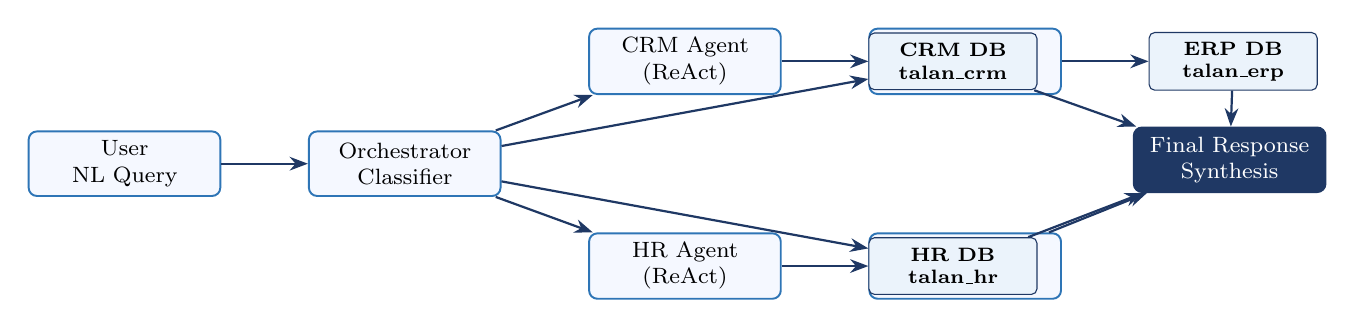
\begin{tikzpicture}[
  font=\footnotesize,
  node distance=0.6cm and 1.1cm,
  box/.style={draw=talanblue,fill=talangray,rounded corners=3pt,
    minimum width=2.3cm,minimum height=0.82cm,
    text width=2.2cm,align=center,line width=0.7pt},
  dark/.style={draw=talannavy,fill=talannavy,rounded corners=3pt,
    minimum width=2.3cm,minimum height=0.82cm,
    text width=2.2cm,align=center,line width=0.7pt,text=white},
  db/.style={draw=talannavy,fill=talanlight,rounded corners=2pt,
    minimum width=2.0cm,minimum height=0.72cm,
    text width=1.9cm,align=center,font=\scriptsize\bfseries},
  arr/.style={-Stealth,talannavy,thick}
]
  % Input & orchestrator
  \node[box]                        (user)  {User\\ NL Query};
  \node[box,right=of user]          (orch)  {Orchestrator\\ Classifier};
  % Agents (staggered)
  \node[box,above right=0.45cm and 1.1cm of orch] (crm) {CRM Agent\\ (ReAct)};
  \node[box,right=1.1cm of crm]                   (erp) {ERP Agent\\ (ReAct)};
  \node[box,below right=0.45cm and 1.1cm of orch] (hr)  {HR Agent\\ (ReAct)};
  \node[box,right=1.1cm of hr]                    (rag) {RAG Agent\\ (Vector)};
  % Databases
  \node[db,right=of crm] (dbcrm) {CRM DB\\ talan\_crm};
  \node[db,right=of erp] (dberp) {ERP DB\\ talan\_erp};
  \node[db,right=of hr]  (dbhr)  {HR DB\\ talan\_hr};
  % Synthesis
  \node[dark,below right=0.4cm and 0.9cm of erp] (synth)
    {Final Response\\ Synthesis};
  % Arrows
  \draw[arr] (user)--(orch);
  \draw[arr] (orch)--(crm); \draw[arr] (orch)--(erp);
  \draw[arr] (orch)--(hr);  \draw[arr] (orch)--(rag);
  \draw[arr] (crm)--(dbcrm); \draw[arr] (erp)--(dberp);
  \draw[arr] (hr)--(dbhr);
  \draw[arr] (dbcrm)--(synth); \draw[arr] (dberp)--(synth);
  \draw[arr] (dbhr)--(synth);  \draw[arr] (rag)--(synth);
\end{tikzpicture}
\caption{TIEA market analysis pipeline: from natural-language input to multi-source synthesized
  response}
\label{fig:pipeline}
\end{figure}

% ─────────────────────────────────────────────────────────────
\subsection{Strategic Positioning of TIEA in the Market}
% ─────────────────────────────────────────────────────────────

\subsubsection{Positioning Matrix}

Based on the competitive analysis and gap quantification, TIEA is positioned as a
\textbf{high-intelligence, low-lock-in} solution (Figure~\ref{fig:positioning}) -- contrasted with
commercial platforms that offer moderate intelligence within a proprietary ecosystem, and raw LLM
frameworks that offer maximum flexibility at the cost of integration effort.

\begin{figure}[H]
\centering
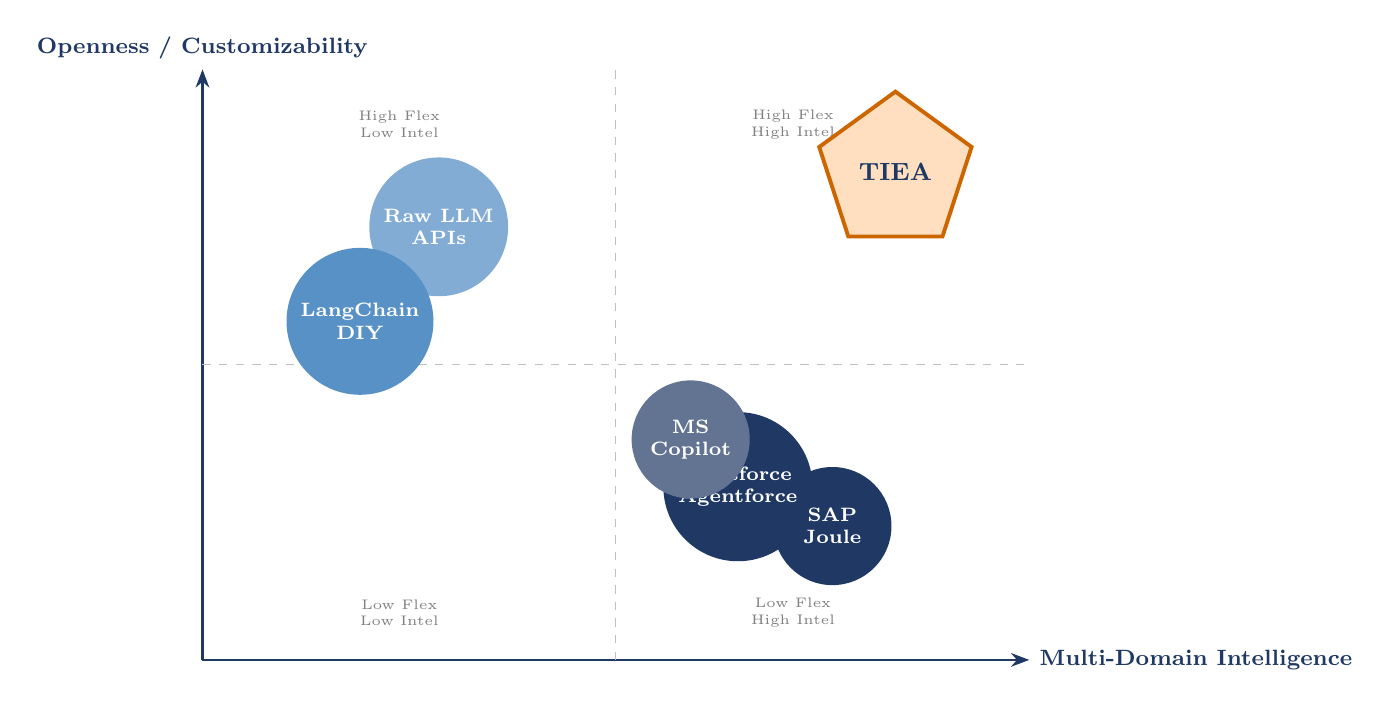
\begin{tikzpicture}[font=\small]
  % Axes
  \draw[-Stealth,thick,talannavy] (0,0)--(10.5,0)
    node[right,font=\footnotesize]{\textbf{Multi-Domain Intelligence}};
  \draw[-Stealth,thick,talannavy] (0,0)--(0,7.5)
    node[above,font=\footnotesize]{\textbf{Openness / Customizability}};
  % Centre lines
  \draw[dashed,gray!50] (5.25,0)--(5.25,7.5);
  \draw[dashed,gray!50] (0,3.75)--(10.5,3.75);
  % Quadrant labels
  \node[gray,font=\tiny,align=center] at (2.5,6.8) {High Flex\\Low Intel};
  \node[gray,font=\tiny,align=center] at (7.5,6.8) {High Flex\\High Intel};
  \node[gray,font=\tiny,align=center] at (2.5,0.6) {Low Flex\\Low Intel};
  \node[gray,font=\tiny,align=center] at (7.5,0.6) {Low Flex\\High Intel};
  % Competitor bubbles
  \node[circle,fill=talannavy,text=white,minimum size=1.5cm,
        font=\scriptsize\bfseries,align=center] at (8.0,1.7) {SAP\\Joule};
  \node[circle,fill=talannavy,text=white,minimum size=1.5cm,
        font=\scriptsize\bfseries,align=center] at (6.8,2.2) {Salesforce\\Agentforce};
  \node[circle,fill=talannavy!70,text=white,minimum size=1.5cm,
        font=\scriptsize\bfseries,align=center] at (6.2,2.8) {MS\\Copilot};
  \node[circle,fill=talanblue!60,text=white,minimum size=1.3cm,
        font=\scriptsize\bfseries,align=center] at (3.0,5.5) {Raw LLM\\APIs};
  \node[circle,fill=talanblue!80,text=white,minimum size=1.3cm,
        font=\scriptsize\bfseries,align=center] at (2.0,4.3) {LangChain\\DIY};
  % TIEA star (drawn as a thick circle to avoid shape library issues)
  \node[regular polygon,regular polygon sides=5,draw=orange!80!black,
        fill=orange!25,line width=1.4pt,
        minimum size=2.0cm,font=\small\bfseries,
        text=talannavy,align=center] at (8.8,6.2) {\textbf{TIEA}};
\end{tikzpicture}
\caption{Strategic positioning matrix: multi-domain intelligence vs.\ openness / customizability}
\label{fig:positioning}
\end{figure}

\subsubsection{Value Proposition Summary}

TIEA occupies a unique position in the intelligent enterprise assistant market, delivering four
core value dimensions that no single competing solution achieves simultaneously
(Table~\ref{tab:value-prop}).

\begin{table}[H]
\centering
\caption{TIEA's Four-Pillar Value Proposition}
\label{tab:value-prop}
\renewcommand{\arraystretch}{1.6}
\begin{tabularx}{\linewidth}{>{\bfseries\color{talannavy}}l X}
\toprule
\rowcolor{talannavy}
\color{white}\textbf{Pillar} & \color{white}\textbf{Description} \\
\midrule
\rowcolor{talangray}
Unified Intelligence &
Single conversational interface over HR, CRM, and ERP data, enabling cross-domain
queries that are impossible in any commercial solution. \\
Openness \& Control &
Built entirely on open-source components (FastAPI, LangGraph, PostgreSQL,
ChromaDB), enabling full customization, self-hosting, and zero vendor lock-in. \\
\rowcolor{talangray}
Role-Aware Access &
Integrated JWT authentication with a three-tier role model
(employee\,/\,manager\,/\,admin) enforced at the agent level,
ensuring data governance without external IAM dependencies. \\
Economic Accessibility &
Total infrastructure cost is compatible with the free tier of available LLM
APIs, making TIEA deployable without enterprise-scale software budgets. \\
\bottomrule
\end{tabularx}
\end{table}

% ─────────────────────────────────────────────────────────────
\subsection{Conclusion of the Market Analysis}
% ─────────────────────────────────────────────────────────────

The market analysis conducted as part of this project confirms a twofold finding.

First, the global enterprise software market is undergoing a structural transition toward
AI-augmented, conversational interfaces, with the AI-in-enterprise-applications segment projected
to grow at over 31\% CAGR through 2028.
The demand for natural-language access to enterprise data is clearly established: 67\% of enterprise
decision-makers identify this capability as a top-three operational priority.

Second, the specific sub-market of intelligent assistants for heterogeneous, multi-domain enterprise
stacks remains effectively unaddressed by commercial vendors, whose offerings are tightly bound to
their proprietary ecosystems.
No existing commercial solution scores above~5 out of~11 on the criteria matrix in
Table~\ref{tab:comparison}, confirming the structural whitespace that TIEA targets.

This gap defines both the strategic rationale and the functional scope of TIEA.
Market analysis is not merely a contextual exercise conducted prior to development: it is an
ongoing, built-in capability of the system, enabling managers, directors, and analysts to query
their CRM pipeline, ERP financials, and HR workforce data through a single natural-language
interface -- and to synthesize cross-domain insights previously accessible only through manual,
multi-step reporting processes.

The following sections elaborate the technical architecture and implementation of TIEA, grounded
in the requirements identified through this market analysis.

% ============================================================
\end{document}
% ============================================================
ough 2028.
The demand for natural-language access to enterprise data is clearly established: 67\% of enterprise
decision-makers identify this capability as a top-three operational priority.

Second, the specific sub-market of intelligent assistants for heterogeneous, multi-domain enterprise
stacks remains effectively unaddressed by commercial vendors, whose offerings are tightly bound to
their proprietary ecosystems.
No existing commercial solution scores above~5 out of~11 on the criteria matrix in
Table~\ref{tab:comparison}, confirming the structural whitespace that TIEA targets.

This gap defines both the strategic rationale and the functional scope of TIEA.
Market analysis is not merely a contextual exercise conducted prior to development: it is an
ongoing, built-in capability of the system, enabling managers, directors, and analysts to query
their CRM pipeline, ERP financials, and HR workforce data through a single natural-language
interface -- and to synthesize cross-domain insights previously accessible only through manual,
multi-step reporting processes.

The following sections elaborate the technical architecture and implementation of TIEA, grounded
in the requirements identified through this market analysis.

% ============================================================
\end{document}
% ============================================================
